W problemie ucztujących filozofów pewna liczba filozofów siedzi przy okrągłym stole i każdy z nich na zmianę albo myśli, albo je. Między filozofami na stole są położone widelce, po jednym między każdą parą filzofów. Aby jeść, filozof musi najpierw podnieść dwa widelce z obu stron. Każdy widelec może być w danym momencie podniesiony lub używany przez co najwyżej jednego filozofa. Problem polega na zaprojektowaniu takiej procedury postępowania dla każdego filozofa (czyli algorytmu rozproszonego), żeby mógł on w nieskończoność na zmianę myśleć i jeść.

\begin{figure}[H]  
    \centering
    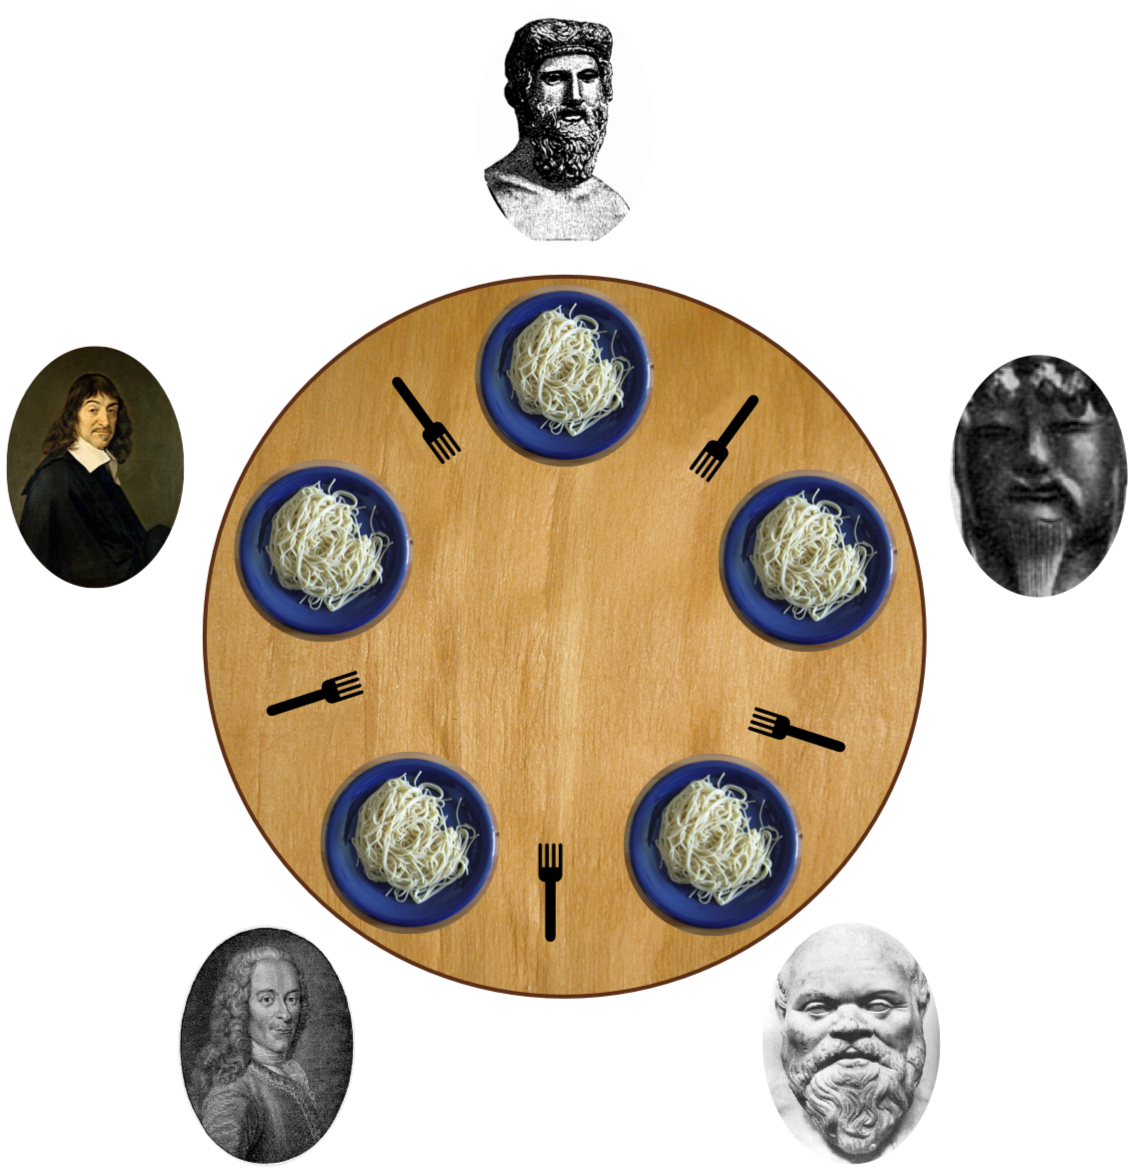
\includegraphics[width=10cm]{chapters/sysopy/filozofowie/An_illustration_of_the_dining_philosophers_problem.png}
\caption{bdesham, User:Belbury, CC BY 3.0, \url{https://creativecommons.org/licenses/by/3.0}, Wikimedia Commons; Ilustracja problemu filozofów}
\end{figure}

Algorytm może być niepoprawny pod względem \textbf{bezpieczeństwa}, jeśli może doprowadzić do deadlocka, na przykład gdy w tym samym momencie każdy filozof podniesie lewy widelec i zacznie czekać na dostępność prawego widelca. 

Algorytm może być niepoprawny pod względem \textbf{żywotności}, jeśli może dojść do takiej sytuacji, że któryś filozof nigdy nie doczeka się obu widelców. Rozwiązanie polegające na numeracji widelców i podnoszeniu ich tylko w odpowiedniej kolejności rozwiązuje problem deadlocków, ale nie gwarantuje żywotności, ponieważ widelec o najmniejszym numerze jest podnoszony w pierwszej kolejności przez dwóch filozofów.

Rozwiązanie:
\begin{itemize}
\item Każdy widelec jest w każdym momencie przez kogoś trzymany.
\item Początkowy przydział widelców nie jest symetryczny, czyli nie jest tak, że każdy trzyma prawy widelec lub każdy trzyma lewy widelec.
\item Każdy filozof po zakończeniu jedzenia przekazuje równocześnie oba widelce do obu sąsiadów
\end{itemize}

Utrzymujemy niezmiennik, że przydział widelców nie jest symetryczny. Przydział nie jest symetryczny wtedy i tylko wtedy, gdy przynajmniej jeden filozof trzyma oba widelce. Po zjedzeniu, filozof oddaje równocześnie oba widelce, więc nowy przydział też nie jest symetryczny.

Skoro przydział nigdy nie jest symetryczny, to zawsze przynajmniej jeden filozof może jeść, więc deadlock jest niemożliwy.

Załóżmy nie wprost, że któryś filozof X nigdy nie doczeka się widelca od sąsiada Y. Zatem Y trzyma widelec po stronie X i sam nigdy nie doczeka się widelca z drugiej strony, bo gdyby się doczekał, to w końcu by zjadł i oddał widelec sąsiadowi X. Kontynuując w ten sposób można pokazać indukcyjnie że przydział jest symetryczny, co jest sprzeczne z niezmiennikiem. Zatem każdy filozof kiedyś doczeka się obu widelców.